\documentclass[11pt,a4paper]{article}
\usepackage{fontspec}
\usepackage{amsmath,amssymb}
\usepackage{geometry}
\usepackage{tikz}
\usetikzlibrary{angles,quotes,calc}

\setmainfont{Liberation Serif}
\setsansfont{Liberation Sans}
\geometry{margin=1.55cm}

\definecolor{accent}{HTML}{9F1239}
\definecolor{ink}{HTML}{1C1917}
\definecolor{guide}{HTML}{78716C}
\color{ink}

\pagestyle{empty}
\setlength{\parindent}{0pt}
\setlength{\parskip}{0.45em}

\newcommand{\boardtitle}[1]{%
  {\sffamily\bfseries\large #1}%
  \par\vspace{0.15em}{\color{accent}\rule{\textwidth}{1.1pt}}\par\vspace{0.55em}%
}

\begin{document}

\begin{center}
  {\sffamily\bfseries\LARGE Правилни петоугао}\\[0.25em]
  {\color{guide} лекција са табле \textemdash\ текст и цртежи}
\end{center}

\vspace{0.4em}
\boardtitle{Нацртати правилни петоугао уписан у кружницу полупречника \(r\).}

\begin{minipage}[t]{0.48\textwidth}
\vspace{0pt}
Цртамо полупречник:
\begin{center}
\begin{tikzpicture}[baseline]
  \draw (0,0) -- (2.4,0);
  \draw (0,-0.08) -- (0,0.08);
  \draw (2.4,-0.08) -- (2.4,0.08);
  \node[above] at (1.2,0) {\(r\)};
\end{tikzpicture}
\end{center}

Рачунамо углове карактеристичног \(\triangle\):
\[
\alpha=\frac{360^{\circ}}{n},
\qquad
x=90^{\circ}-\frac{180^{\circ}}{n}.
\]
За петоугао је \(n=5\):
\[
\alpha=\frac{360^{\circ}}{5}=72^{\circ},
\qquad
x=54^{\circ}.
\]

\begin{center}
\begin{tikzpicture}[line join=round,scale=1.05]
  \coordinate (A) at (0,0);
  \coordinate (B) at (3.1,0);
  \coordinate (C) at (1.55,2.05);
  \draw (A) -- (B) -- (C) -- cycle;
  \node[below left] at (A) {\(x\)};
  \node[below right] at (B) {\(x\)};
  \node[above] at (C) {\(\alpha\)};
\end{tikzpicture}
\end{center}

Цртамо карактеристични \(\triangle\), око њега описујемо кружницу и помоћу шестара тражимо остала тјемена многоугла.
\end{minipage}\hfill
\begin{minipage}[t]{0.50\textwidth}
\vspace{0pt}
\begin{center}
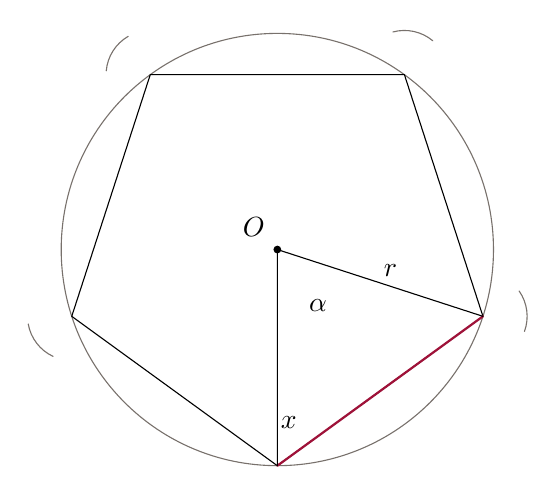
\begin{tikzpicture}[line cap=round,line join=round,scale=1.22]
  \def\R{2.25}
  \coordinate (O) at (0,0);
  \draw[guide] (O) circle[radius=\R];
  \foreach \i in {0,...,4}
    \coordinate (V\i) at ({-90+\i*72}:\R);
  \draw (V0) -- (V1) -- (V2) -- (V3) -- (V4) -- cycle;
  \draw[accent,thick] (V0) -- (V1);
  \draw (O) -- (V0) (O) -- (V1);
  \fill (O) circle[radius=1.15pt];
  \node[above left=1pt] at (O) {\(O\)};
  \node at ({-54}:0.72) {\(\alpha\)};
  \node at ($(V0)+(75:0.46)$) {\(x\)};
  \node[above] at ($(O)!0.55!(V1)$) {\(r\)};
  \foreach \i/\a in {1/-20,2/50,3/120,4/190}
    \draw[guide] ([shift={({\a}:0.46)}]V\i) arc[start angle=\a,end angle=\a+55,radius=0.46];
\end{tikzpicture}
\end{center}
\end{minipage}

\vspace{1.1em}
\boardtitle{Конструкција и цртање правилног многоугла}

\textbf{Примјер.} Нацртати правилни петоугао чија страница има дужину \(3\,\mathrm{cm}\).

\begin{minipage}[t]{0.42\textwidth}
\vspace{0.2em}
Дата је страница:
\begin{center}
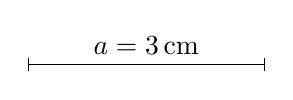
\begin{tikzpicture}
  \draw (0,0) -- (3,0);
  \draw (0,-0.08) -- (0,0.08);
  \draw (3,-0.08) -- (3,0.08);
  \node[above] at (1.5,0) {\(a=3\,\mathrm{cm}\)};
\end{tikzpicture}
\end{center}

Унутрашњи угао правилног петоугла је \(108^{\circ}\), а централни угао описане кружнице је \(72^{\circ}\). Шестаром преносимо страницу \(a\) по кружници док не затворимо свих пет тјемена, па спајамо тјемена.
\end{minipage}\hfill
\begin{minipage}[t]{0.56\textwidth}
\vspace{0pt}
\begin{center}
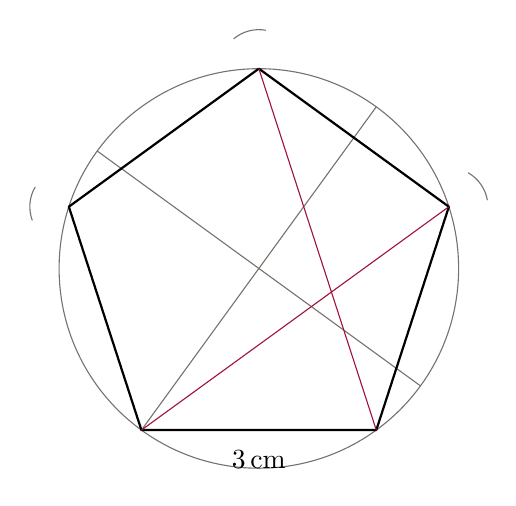
\begin{tikzpicture}[line cap=round,line join=round,scale=1.18]
  \def\R{2.15}
  \coordinate (O) at (0,0);
  \draw[guide] (O) circle[radius=\R];
  \draw[guide] ($(O)+(-126:\R)$) -- ($(O)+(54:\R)$);
  \draw[guide] ($(O)+(-36:\R)$) -- ($(O)+(144:\R)$);
  \foreach \i in {0,...,4}
    \coordinate (W\i) at ({-126+\i*72}:\R);
  \draw[thick] (W0) -- (W1) -- (W2) -- (W3) -- (W4) -- cycle;
  \draw[accent] (W0) -- (W2) (W1) -- (W3);
  \node[below=4pt] at ($(W0)!0.5!(W1)$) {\(3\,\mathrm{cm}\)};
  \foreach \i/\a in {2/10,3/80,4/150}
    \draw[guide] ([shift={({\a}:0.42)}]W\i) arc[start angle=\a,end angle=\a+50,radius=0.42];
\end{tikzpicture}
\end{center}
\end{minipage}

\end{document}
